\documentclass{amsart}
\usepackage{graphicx,amsfonts,amsthm,amsmath,amssymb,enumerate,enumitem,xcolor,commath,hyperref} % Required for inserting images
\usepackage{geometry}[margin=1in]
\usepackage{biblatex}[sorting=none]

\title{An Introduction to Computational Stochastic PDEs\\ Exercises: Chapter 1}
\author{Chris DuPre }
\date{April 2024}

\theoremstyle{plain}
\newtheorem{thm}{Theorem}[section]
\newtheorem{lem}[thm]{Lemma}
\newtheorem{prop}[thm]{Proposition}
\newtheorem*{cor}{Corollary}

\theoremstyle{definition}
\newtheorem{defn}{Definition}[section]
\newtheorem{conj}{Conjecture}[section]
\newtheorem{exmp}{Example}[section]
\newtheorem{exer}{Exercise}[section]

\newcommand{\R}{\mathbb{R}}
\newcommand{\C}{\mathbb{C}}
\newcommand{\Z}{\mathbb{Z}}
\newcommand{\Q}{\mathbb{Q}}
\newcommand{\N}{\mathbb{N}}
\newcommand{\Hil}{\mathcal{H}}
\newcommand{\E}{\mathcal{E}}

\newcommand{\tcr}[1]{\textcolor{red}{#1}}

\bibliography{Ref}

\begin{document}

\maketitle
\setcounter{section}{1}
\begin{exer}
For a bounded domain $D$, prove that $C\left(\overline{D}\right)$ is complete with respect to the supremum
norm $\|u\|_{\infty} = \sup_{x \in D} \abs{u(x)}$. By constructing a suitable Cauchy sequence, show that
$C\left(\overline{D}\right)$ is not complete with respect to the $L^{2}(D)$ norm. 
\end{exer}
\begin{proof}
    First, note that $\overline{D}$ is bounded as $D$ is bounded. Thus by Heine-Borel, $\overline{D}$ is compact. As continuous functions achieve their supremeum on compact sets, each $f_k$ is bounded. Define $M_n := \sup_{y\in \overline{D}} f(y)$. We first claim that $f_k$ as a sequence is uniformly bounded. To see this, note that as $f_k$ is Cauchy, there exists an $N$ such that for all $m,l\geq N$ we have that $\|f_m-f_l\|_{\infty} < 1.$ We thus have that $\sup_{y\in \overline{D}} \abs{f_l(y)} \leq M_N + 1.$ We thus have that $\sup_{k\in \N, x\in \overline{D}}\abs{f_k(x)} \leq \max\left\{\{M_k\}_{k=1}^{N}\right\}+1.$
    \par 
    As these are uniformly bounded, in particular for every $y\in \overline{D}$, we have that $f_k(y)$ is bounded and Cauchy. As $\R$ is complete, it must converge. For every $x\in \R$, define
    $$f(x) = \lim_{k\to \infty} f_k(x).$$
    We claim that $\lim_{k\to \infty} \sup_{y\in D} \abs{f_k(y)-f(y)} = 0$, (we do not use the norm as a-priori we do not know this function is continuous). As $\abs{\cdot}$ and subtraction are continuous, it is clear that for every $y \in \overline{D}$ that
    $$\abs{f_{k}(y)-f(y)} \leq\lim_{m\to \infty}\abs{f_{k}(y)-f_{m}(y)} \leq \limsup_{m\to \infty} \|f_k -f_m\|_{\infty}.$$
    As the right hand side is independent of $y$, we may take the supremum over the right hand side. For all $\varepsilon > 0$, there exists an $N$ such that the right hand side is less than $\varepsilon$ if $k=N$. As $\varepsilon$ is arbitrary, it is clear that 
    $$lim_{k\to \infty} \sup_{y\in D} \abs{f_k(y)-f(y)} = 0.$$
    \par We now claim that $f$ is continuous. To see this, note
    $$\abs{f(x)-f(y)}\leq \abs{f(x)-f_k(x)}+\abs{f_k(x)-f_k(y)}+\abs{f_k(y)-f(y)}.$$
    By the previous statement, there exists a $k$ such that the first and last terms are less than $\varepsilon/3$ for all $x,y\in\overline{D}.$ As $f_k$ is then continuous, there exists $\delta > 0$ such that if the distance between $x,y$ is less than $\delta$ we have that the middle term is less than $\varepsilon/3$. Thus $f$ is continuous.
    \par As a counter example for $L^2$, consider
    $$f_k(x) = \begin{cases}
        0 & -2\leq x \leq -1-\frac{1}{k}\\
        \frac{k(x+1)+1}{2}& \abs{x+1}\leq \frac{1}{k}\\
        1 & \abs{x}\leq 1-\frac{1}{k}\\
        \frac{k(1-x)+1}{2}& \abs{x-1}\leq \frac{1}{k}\\
        0 & 1+\frac{1}{k}\leq x\leq 2
    \end{cases}$$
    \begin{figure}[h!]
        \centering
        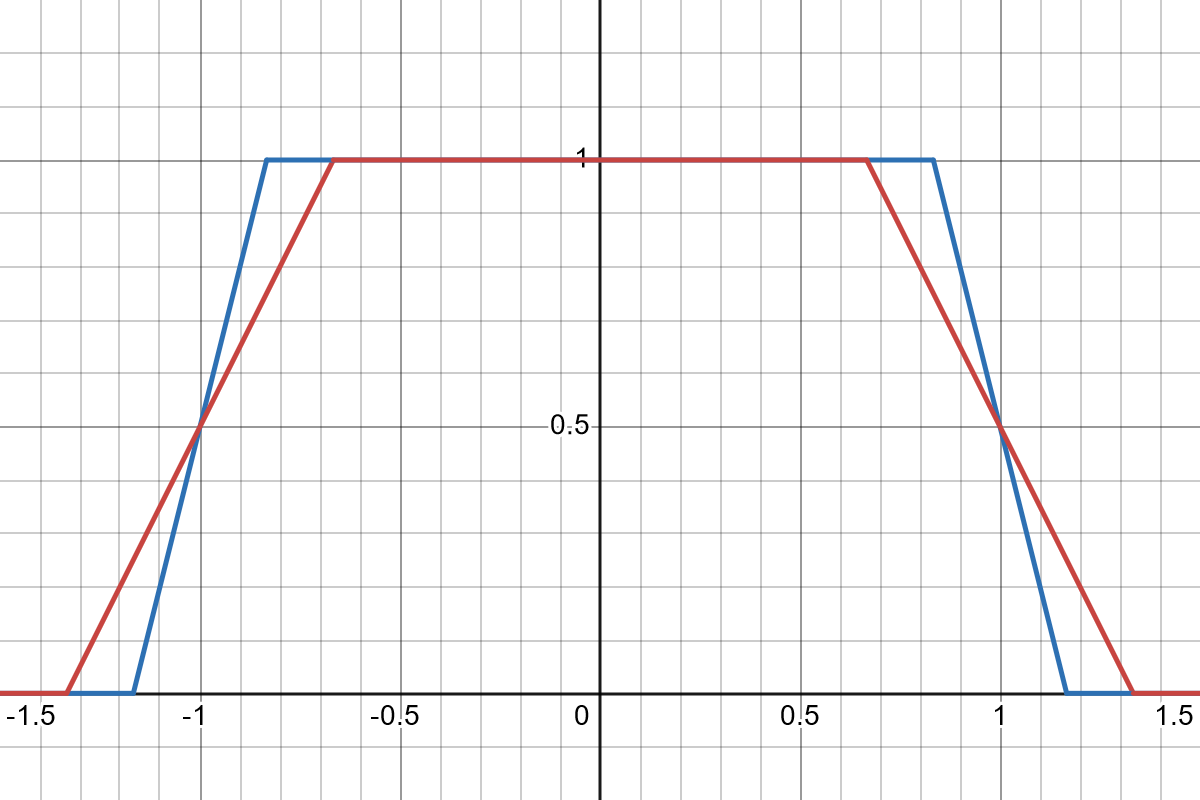
\includegraphics[width=0.5\linewidth]{Chapter 1/Photos/Problem1Counter.png}
        \caption{Depiction of counter example family. Red is $k=3$. Blue is $k=7$.}
        \label{fig:Problem_1_counter}
    \end{figure}
    This family is clearly continuous on $[-2,2].$ It is also clearly Cauchy, as in particular
    $$\|f_k - f_m\|_{L^2} \leq \frac{2}{\min_{m,k}}.$$
    However, this sequence converges to $\mathbf{1}_{[-1,1]}$ which is not continuous and therefore not in the space. Thus we have a Cauchy sequence which does not converge and the space is not complete
\end{proof}

\begin{exer}
    Let $\left(X,\mathcal{F},\mu \right)$ be a complete measure space, $Y$ be a Banach space, and $f : X \to Y$ a measurable function. Show that $f = g$ a.s. implies that g is measurable. Give an example to show that the completeness assumption on the measure space is necessary.
\end{exer}
\begin{proof}
Note that $f= g$ a.s. implies that there exists a measurable null set $N$ such that $f=g$ on $N^C$. Let $B$ be measurable and consider $g^{-1}(B).$ Then clearly $g^{-1}(B) = g^{-1}(B)\cap N \cup g^{-1}(B) \cap N^C = g^{-1}(B)\cap N \cup f^{-1}(B) \cap N^C.$ By completeness, $g^{-1}(B)\cap N$ is measurable. Thus $g^{-1}(B)$ is a finite union of measureable sets and is thus measureable. 
\par To see that completeness is neccesary. Consider $X = \{1,2,3\}, \mathcal{F} = \{\empty,\{1\},\{2,3\},\{1,2,3\}\}$ with $\mu\left(\{1\}\right) = 1, \mu\left(\{2\}\right)=\mu\left(\{3\}\right).$ Let $f$ be defined as $f(1) = f(2) = 0, f(3) = 0$ and $g(1)=g(3) = 1, g(2) = 0$. Note that $f = g$ a.s. with $N = \{2,3\}$ and $f$ is measureable but $g$ is not.  
\end{proof}

$$\int_{X} \|u(x)\|_{Y} dx < \infty.$$
\begin{exer}
   Using Definition 1.2.1 in \cite{lord2014introduction}, prove that if $u:X\to Y$ is integrable then 
        $$\int_{X} \|u(x)\|_{Y} dx < \infty.$$
\end{exer}
\begin{proof}
    Note that 
    \begin{align*}
        \int_{X} \|u(x)\|_{Y} dx &\leq \int_{X} \|u(x)-u_k(x)\|_{Y} dx + \int_{X} \|u_k(x)\|_{Y} dx \\
        & = \int_{X} \lim_{m\to \infty} \|u_m(x)-u_k(x)\|_{Y} dx + \int_{X} \|u_k(x)\|_{Y} dx \\
        & \leq \liminf_{m}\int_{X} \|u_m(x)-u_k(x)\|_{Y} dx+ \int_{X} \|u_k(x)\|_{Y} dx.
    \end{align*}
    The last inequality follows by Fatou's lemma. 
    For $k$ sufficiently large , the first term is bounded by $1$ by Definition 1.2.1. By the definition of simple functions, the second is also bounded. Thus the term on the left is bounded as well.
\end{proof}

\begin{exer}
\tcr{Newline}
    \begin{enumerate}[label=\alph*.]
        \item If $u:\R\to\R$ is measurable, define simple functions $u_n$ such that $u_n(x) \to u(x)$ for all $x\in\R.$
        \item If $G\in C\left(\R\times \R\right)$, define simple functions of the form
        $$\sum_{j,k=1}^{N} G(x_j,x_k)\mathbf{1}_{\mathcal{F}_j}\mathbf{1}_{\mathcal{F}_k}$$
        for $x_j\in\R, F_j \in \mathcal{B}\left(\R\right)$, such that $G_j\to G$ point-wise as $N\to \infty.$
    \end{enumerate}
\end{exer}
\begin{proof}\tcr{Somehow}
    \begin{enumerate}[label=\alph*.]
        \item Define $\mathcal{F}_{j}^{n} = u^{-1}\left(\left[\frac{j}{n},\frac{j+1}{n}\right)\right)\cap\left[-n,n\right], -n^2 \leq j \leq n^2$ and define:
        $$u_n(x) = \sum_{j=-n^2}^{n^2} \frac{j}{n}\mathbf{1}_{\mathcal{F}_{j}^{n}}.$$
        It is clear this function is simple as each set is clearly measurable and $\mu\left(\mathcal{F}_j^n\right)\leq 2n$. Consider $x\in \R$. Then for $n\geq \lceil \abs{x}\rceil$, we have that $\abs{u(x)-u_{n}(x)}\leq \frac{1}{n}$ and thus it converges point-wise.
        \item
    \end{enumerate}
\end{proof}

\printbibliography
\end{document}
